	\section{Literature Review}
	\label{sec:litreview}
	
	\paragraph*{} Building on the introduction, which outlined the significance of sustainable innovation in disruptive industries such as clean energy and cultured meat, the literature review critically examines the current state of academic and industry knowledge on how sustainability is managed and implemented within these emerging sectors. While sustainability and disruption are widely discussed in management literature, most analysis remain concentrated at the level of technological feasibility or executive decision making. There is limited understanding of how sustainability is translated into practice within organizations, especially by middle managers who bridge strategic directives and day-to-day operations. This oversight is particularly problematic: while middle managers serve as crucial intermediaries between strategic vision and operational execution, their role in sustainable innovation within disruptive contexts remains largely unexplored (\textcite{Floyd1997}). While these industries offer significant potential for addressing global sustainability challenges, their success depends critically on effective management practices that can navigate high uncertainty and rapid change (\textcite{Christensen1997}).
	
	\paragraph*{} This literature review examines the intersection of management practices and sustainable innovation in disruptive industries, with particular focus on identifying the research gap concerning middle management’s role. By analyzing the distinct challenges within cultured meat and renewable energy sectors, this review establishes the theoretical foundation for understanding how middle managers contribute to sustainability transitions in rapidly evolving industries.
	
	\subsection*{Structure of the Literature Review}
	This literature review examines seven key themes that collectively build the case for studying middle management in sustainable innovation. First, it establishes management’s fundamental role in driving sustainability outcomes. Second, it highlights the current research emphasis on executive leadership. Third, it examines why generic sustainability frameworks may be insufficient for disruptive industries. Fourth, it defines disruption within sustainable innovation contexts. Fifth, it analyzes specific barriers in cultured meat and renewable energy sectors. Sixth, it explores market adoption challenges in translating innovation to impact. Finally, it identifies the research gap regarding middle management’s role in sustainability transitions. Each section synthesizes academic literature and industry evidence to support the need for focused research on middle management in disruptive sustainable industries.
	
	\subsection{The Strategic Role of Management in Corporate Sustainability}
	The integration of sustainability into corporate strategy is increasingly recognized as a cornerstone of long-term organizational success(\textcite{Avery2005}). A growing body of literature emphasizes the critical role of management, particularly top executives, in embedding sustainability principles within business operations. Leadership commitment at the highest levels acts as a catalyst for systemic change, setting the tone for sustainable practices across the organization (\textcite{Waldman2008}). Sustainable leadership entails balancing economic, social, and environmental objectives through comprehensive and adaptive decision-making frameworks (\textcite{Lozano2015}).
	
	\paragraph*{} \citeauthor{Eccles2014} provide empirical evidence through a longitudinal study of “High Sustainability” firms, demonstrating that companies with formal sustainability governance structures such as board-level oversight and executive incentive mechanisms outperform their peers financially over time (\textcite{Eccles2014}). These findings support the argument that top management is not merely a facilitator but a key enabler of effective and enduring sustainability transitions.
	
	\paragraph*{} The scope of managerial influence extends well beyond operational efficiency to encompass the cultivation of an organizational identity rooted in sustainability values. This transformation involves guiding strategic direction, enhancing stakeholder trust and legitimacy, and embedding sustainability principles into corporate DNA (\textcite{Eccles2014, Dyllick2016}). However, successful sustainability integration requires active participation across all hierarchical levels and stakeholder groups, including boards of directors, shareholders, and employees (\textcite{Freeman1984}).
	
	\paragraph*{} Recent studies on small and medium-sized enterprises (SMEs) and startups provide particularly compelling evidence of management’s mediating role in sustainability outcomes. \citeauthor{Madrid2023, Memon2022} demonstrate how management commitment serves as a crucial bridge between sustainability drivers and environmental performance (\textcite{Madrid2023, Memon2022}). When top executives champion environmental values, firms demonstrate a significantly higher likelihood of implementing sustainable practices.
	
	\paragraph*{} In sum, the role of management spanning strategic vision, operational execution, and cultural transformation is indispensable in advancing corporate sustainability agendas and achieving enduring competitive advantage.
	
	\subsection{The Executive-Centric Focus and Its Limitations}
	Despite widespread recognition of management's importance in sustainability, academic research exhibits a pronounced executive-centric bias that limits our understanding of sustainability implementation across organizational levels. The literature predominantly examines senior managers, CEOs, and boards of directors who set strategic direction and initiate sustainability initiatives, while systematically overlooking contributions from middle and lower management levels.
	
	\paragraph*{} This executive focus has established a prevailing narrative rooted in top-down leadership models. Upper Echelons Theory (UET) has gained prominence in sustainability research, explaining how top managers' demographic, cognitive, and experiential characteristics including age, tenure, education, and value orientation influence corporate social responsibility (CSR) and sustainable innovation outcomes (\textcite{Waldman2008, Ioannou2015}). Researchers emphasize how top management teams shape organizational culture, allocate sustainability resources, and foster cross-sector collaboration, particularly when leaders adopt systems thinking approaches (\textcite{Dyllick2016}).
	
	\paragraph*{} Supporting this trend, \citeauthor{keil2024c} found that institutionalized sustainability responsibilities like board-level oversight and top-down governance structures are among the strongest predictors of successful sustainability practices(\textcite{keil2024c}). Similarly, research on SMEs consistently highlights the central role of owner or top level managers in driving environmental performance (\textcite{kustbash}). In contrast studies involving larger corporations focus on how executive compensation tied to environmental metrics drives superior financial and environmental performance (\textcite{Eccles2014}).
	
	\paragraph*{} However, this executive-centric perspective creates a substantial gap in understanding how sustainability strategies are operationalized. Middle managers translate strategic sustainability goals into practical actions. They coordinate cross-functional teams, allocate operational resources, and manage emergent challenges during implementation. Omitting middle management from academic discourse limits comprehension of how organizations embed sustainability in everyday practices and across hierarchical layers.
	
	\paragraph*{} This limitation becomes particularly problematic when examining SMEs, where organizational structures tend to be flatter and distributed leadership is much more common. Even in these contexts, research frequently attributes sustainability outcomes solely to top executives, obscuring the grassroots engagement and distributed leadership that drive sustainability implementation (\textcite{birkinshaw2010}).
	
	\subsection{Generalized Frameworks and Theoretical Limitations}
	A recurring limitation in the current sustainability literature is the tendency to rely on broad, generalized theoretical models that lack contextual specificity. Frameworks such as the triple bottom line and stakeholder theory are commonly applied due to their wide applicability, but their utility diminishes in specific or emerging industry settings(\textcite{Donaldson1995, Elkington1997}). While these models offer valuable conceptual guidance, they often fail to capture the complexities of specific organizational contexts. \citeauthor{kustbash} argue that theories derived from large corporate environments do not easily translate to smaller firms or disruptive sectors, noting that "no coherent theory exists about the drivers of corporate sustainability in SMEs" (\textcite{kustbash}). Similarly, \citeauthor{keil2024a} observe that critical variables such as leadership behaviours, organizational culture, and employee engagement are frequently studied in isolation, resulting in fragmented insights rather than an integrated understanding of sustainable performance (\textcite{keil2024a}). 

	\paragraph*{} This theoretical generality extends to empirical research, which emphasizes macro-level factors like national policies and technological innovations while overlooking organizational implementation processes. Studies on renewable energy focus on grid infrastructure and regulatory mechanisms, neglecting managers' day-to-day operational practices (\textcite{IRENA2020}). Similarly, cultured meat research prioritizes technical processes and regulatory hurdles over leadership dynamics and managerial roles (\textcite{Bryant2020}). This creates a critical blind spot in understanding how sustainability strategies are operationalized at various managerial levels, particularly middle management, which bridges executive strategy and front line implementation.
	
	\subsection{Conceptualizing Disruptive Industries in Sustainability Literature}
	\label{sec:ConceptualizingDisruptive}
	Recent scholarship has advanced several frameworks for categorizing disruptive industries, focusing not alone on technological novelty or business model innovations but also factors like industry maturity, regulatory complexity, and the nature of business model innovation (\textcite{Tushman1986}). For example, sectors like cultured meat and synthetic biology are often categorized as emerging disruptive industries as they are categorized by high uncertainty, nascent regulatory environments, and foundational technological challenges. In contrast, industries like clean energy or electric vehicles represent maturing disruptive industries, where core technologies are established but scaling and integration into existing markets presents ongoing obstacles (\textcite{Tushman1986}). Classic definitions of disruptive innovation, such as those by \citeauthor{Tushman1986}, emphasize technological discontinuities i.e. radical shifts in products, processes, or value chains. More recent perspectives highlight the importance of scalable, novel approaches that replace traditional industry models (\textcite{Yu2010}). In business theory, disruptive innovation refers to innovations that begin by serving overlooked or under served market segments with simpler, more affordable, and accessible offerings, and eventually displace established market leaders and their sustaining innovations (\textcite{Christensen1997}). These innovations often originate from startups or peripheral market players rather than incumbents, and their initial market appeal may not generate sufficient profit to attract attention from larger firms. Over time, however, they reshape the competitive landscape by targeting non consumers or over served customers with "good enough" solutions.
	
	\paragraph*{} The success of disruptive innovations depends not only on technology but on developing business models capable of redefining value delivery (\textcite{Chesbrough2007}). This highlights that effective management in disruptive industries requires a strategic orientation toward adaptability, innovation, and foresight beyond technical proficiency. However, disruptive sectors introduce unique challenges including regulatory uncertainty, consumer skepticism, and high capital intensity, which remain under explored in sustainability research (\textcite{Wustenhagen2007}).
	
	\paragraph*{} The transformational nature of disruptive sectors implies that traditional management approaches may be inadequate. Managers must innovate at both technology and business model levels, proactively monitoring emerging trends, responding to market signals, and cultivating novel approaches to customer value creation under rapid change and uncertainty (\textcite{Teece2007}).
	
	\paragraph*{} This literature-based typology provides a useful analytical lens for comparing managerial practices and sustainability strategies across different disruptive contexts. By situating the present’s study’s sectors within these broader categories, it becomes possible to generalize insights regarding the operationalization of sustainability and the unique role of middle management in navigating sector-specific barriers and opportunities. 
	
	\subsection{Barriers to Sustainability in Cultured Meat and Clean Energy}
	Cultured meat and clean energy industries both aim to advance sustainability but face different types of barriers, reflecting their relative levels of maturity and technological pathways. Understanding these differences is crucial to assessing how middle managers operate within them.
	
	\subsubsection{Cultured Meat}
	The cultured meat industry presents significant potential for sustainable food systems by reducing reliance on conventional animal agriculture. However, it faces substantial technological, economic, and social barriers to scale and adoption. Technologically, the industry remains dependent on high energy input and growth media derived from animal serum or synthetic compounds, which undermines sustainability claims (\textcite{Specht2023, Post2020}). Additionally, cost-effective scalability remains elusive due to inefficient bioreactor designs, high input costs, and the lack of commercially viable scaffolds for structured meat production (\textcite{Bodiou2020}). Other unresolved technical challenges include replicating the nutritional profile of conventional meat and mitigating contamination risks in large-scale operations.
	
	\paragraph*{} From an economic standpoint, high production costs and capital-intensive processes limit commercial viability. Infrastructure remains nascent, and supply chains for bioreactors, culture media, and skilled labor are underdeveloped (\textcite{Stephens2018}). Social and ethical dimensions also pose challenges. Concerns about unnaturalness, food safety, and religious or dietary restrictions (e.g., halal, kosher) impede consumer acceptance (\textcite{Bryant2020}). Furthermore, the potential displacement of traditional livestock farming communities raises questions about equitable transitions in the food economy.
	
	\paragraph*{} Regulatory uncertainty compounds these challenges. To date, only a few countries, including Singapore and the United States, have authorized cultured meat for sale, and harmonized global standards are lacking (\textcite{SFA2020, FDA2023}). Finally, environmental concerns persist, particularly regarding waste management from spent culture media and the disposal of single-use bioreactor components. These internal, science-driven challenges mean that middle managers in the cultured meat sector often work under conditions of technological ambiguity and evolving public trust, requiring flexible decision-making and strong communication strategies.
	
	\subsubsection{Clean Energy}
	The clean energy sector is a cornerstone of decarbonization strategies but faces its own complex set of technological, economic, and political barriers. The intermittent nature of solar and wind energy requires robust and scalable energy storage systems, yet current battery technologies face efficiency, cost, and material constraints (\textcite{OECD2022, IEA2021}). Additionally, existing energy grids are often ill-equipped to manage fluctuating supply and demand, particularly in developing regions where infrastructure is outdated or lacking.
	
	\paragraph*{} High upfront capital expenditure remains a central obstacle to deployment, especially for small and medium-sized enterprises (SMEs), which may lack access to financing mechanisms (\textcite{OECD2022}). Market dominance by fossil fuel incumbents further inhibits the competitiveness of clean energy firms (\textcite{IRENA2017}). Socially, job displacement in traditional energy sectors (e.g., coal, oil) necessitates targeted reskilling programs to ensure a just energy transition.
	
	\paragraph*{} Policy fragmentation and lengthy permitting procedures create additional delays and investor uncertainty. Even in supportive jurisdictions, regulatory bottlenecks slow the expansion of renewable installations (\textcite{OECD2022}). Environmental concerns also persist, such as habitat disruption from wind farms or solar arrays, and the ecological impact of rare earth mining required for clean energy technologies (\textcite{IEA2021}). Furthermore, supply chain vulnerabilities inked to geopolitically sensitive raw materials pose ongoing risks to deployment. In contrast to the internal development focus of cultured meat, middle managers in clean energy must balance external coordination, regulatory navigation, and implementation logistics, often under the pressure of policy shifts and capital-intensive project execution.
	
	\subsubsection{Cross-Sector Insights}
	The contrast between these two sectors highlights a valuable comparative angle: while cultured meat managers are likely to focus on foundational R\&D innovation and managing consumer perceptions, clean energy managers engage with scaling technologies and navigating policy or infrastructure barriers. This distinction shapes how sustainability strategies are enacted on the ground and underscores the importance of context-specific middle management approaches in disruptive environments.
	
	\paragraph*{} The influence of social acceptance emphasizes the need for transparent communication strategies and participatory policy making. Technological advancement alone is insufficient; both sectors must also innovate in business models, supply chains, and stakeholder engagement. Addressing these complex, multi-level challenges will require coordinated policy support, cross-sector learning, and holistic system thinking that goes beyond technological innovation to include governance, equity, and long-term impact. These differences not only influence the types of barriers faced but also shape the pathways to market adoption and organizational learning themes explored in the following sections.
	
\begin{table}[h!]
	\centering
	\caption{Summary of Barriers to Sustainable Development in Cultured Meat and Clean Energy}
	\label{tab:barriers_summary}
	\begin{tabularx}{\textwidth}{@{}lXX@{}}
		\toprule
		\textbf{Barrier Category} & \textbf{Cultured Meat}                                                                     & \textbf{Clean Energy}                                                              \\ \midrule
		Technological             & High energy use, synthetic growth media, scalability, contamination, scaffold R\&D          & Intermittency, storage limitations, outdated grids, material constraints        \\ \addlinespace
		Economic                  & High costs, capital intensity, underdeveloped infrastructure                             & High initial investment, fossil fuel incumbency, access to finance             \\ \addlinespace
		Social/Ethical            & Consumer acceptance (safety, religion, naturalness), rural job displacement              & NIMBYism, demand for transparency, workforce transitions                       \\ \addlinespace
		Regulatory/Policy         & Evolving standards, lack of international harmonization                                  & Policy inconsistency, permitting delays, regulatory uncertainty                \\ \addlinespace
		Infrastructure            & Bioreactor and waste system immaturity                                                   & Grid transmission limits, infrastructure lag in low income regions, supply chain vulnerabilities \\ \addlinespace
		Environmental             & Waste management, emissions from production, resource intensity                          & Land use conflicts, rare earth mining, technology manufacturing impacts        \\ \bottomrule
	\end{tabularx}
\end{table}
	
	\subsection{The Imperative of Market Adoption for Sustainable Innovation}
	Innovation is widely recognized as a crucial catalyst for advancing sustainability goals, driving organizational and technological progress that can simultaneously improve financial performance and generate positive environmental and social impacts (\textcite{Boons2013, Schiederig2012}). Sustainable innovation encompasses the development of new or significantly improved products, processes, technologies, capabilities, and business models that reduce resource consumption while supporting environmental health and community well-being (\textcite{Adams2016}). This innovation ranges from incremental improvements to radical changes that fundamentally reshape business operations, balancing economic, environmental, and social outcomes.
	
	\paragraph*{} However, innovation alone is insufficient; for sustainable technologies to deliver meaningful outcomes, they must achieve broad market penetration. As emphasized by the Good Food Institute (2022), alternative proteins will only become effective climate solutions through wide-scale adoption (\textcite{GFI2022}). Similarly, \citeauthor{Eccles2014} highlight that sustainability performance improves when firms align internal structures such as metrics and decision rights with sustainable outcomes (\textcite{Eccles2014}). Market adoption also depends on broader system level dynamics, including consumer acceptance, institutional pressures, and industry norms (\textcite{Hall2003, Geels2002}).
	
	\paragraph*{} Successfully translating technical innovations into marketable solutions depends on an organization's capacity to operationalize sustainable practices; a responsibility increasingly resting on middle management (\textcite{Rafaeli2022}). They serve as critical enablers of innovation implementation, translating strategic intent into outcomes and navigating organizational resistance (\textcite{birkinshaw2004}). Commercializing sustainable innovations involves overcoming unique challenges related to technology development, market creation, and socio-cultural shifts, requiring collaboration among academic institutions, industries, and governments.
	
	\subsection{Research Gap: Middle Management in Disruptive Sustainability Contexts}
	Despite management's documented importance in driving sustainability initiatives, middle management's role within disruptive sectors remains under explored. They translate strategic visions into operational realities, bridging executives and front line staff while managing resource allocations and ensuring sustainability implementation. However, current literature predominantly focuses on executive-level leadership while neglecting middle management’s crucial operational influence.
	
	\paragraph*{} In disruptive industries like cultured meat and clean energy, understanding how middle managers facilitate or hinder sustainable innovation is vital. These sectors face unique barriers requiring innovative solutions at the operational level. In the clean energy sector, they must navigate scaling renewable infrastructure, grid integration challenges, and complex supply chains while fostering inter-organizational coordination. In the cultured meat sector, they translate scientific breakthroughs into commercially viable production processes, managing operational uncertainties while establishing protocols for contamination control and product consistency under ethical scrutiny and consumer uncertainty.
	
	\paragraph*{} Middle managers are uniquely positioned to drive operational innovation due to their strategic positioning between executive vision and frontline implementation. Their role becomes critical in disruptive sectors due to fast innovation cycles and novel regulatory landscapes. Unlike traditional industries with established practices, middle management in these sectors must interpret sustainability strategies in uncharted territory, amplifying the importance of fostering organizational learning and managing emergent risks.
	
	\subsubsection{Rationale for Comparative Industry Focus}
	This research focuses on cultured meat and clean energy as examples of disruptive sustainability sectors for several strategic reasons. Clean energy represents a relatively mature yet continuously evolving industry crucial for global decarbonization, while cultured meat exemplifies an emerging sector with transformative potential for sustainable food systems. Both sectors share fundamental characteristics including heavy R\&D investment requirements, novel regulatory landscapes, and the imperative to balance sustainability goals with commercial viability.
	
	\paragraph*{} The comparative approach is particularly valuable because these industries' differing maturity levels reveal varied middle management approaches to shared challenges. In the emerging cultured meat sector, middle management must establish initial market footholds while overcoming fundamental production hurdles and consumer skepticism about novel food technologies. Conversely, in the more developed clean energy sector, middle managers focus on optimizing existing processes, managing large-scale infrastructure projects, and navigating established yet complex stakeholder environments.
	
	\paragraph*{} This comparison enables exploration of operational complexity inherent in each sector. The distinct day-to-day operational realities, despite shared foundational characteristics like R\&D intensity, make these sectors ideal for understanding how management approaches vary in driving sustainability within disruptive contexts.
		
	\subsubsection{Research Questions}
	This study addresses two comparative research questions exploring middle management strategies across these sectors:
	\begin{enumerate}
		\item[\textit{i.}] \textbf{Research Question 1:} How do management strategies differ in addressing energy-intensive production challenges in clean energy versus cultured meat?
		
		This question explores anticipated variations in managerial responses to significant technical hurdles. Clean energy’s challenges often involve scaling existing infrastructure and managing intermittency, likely orienting middle management toward optimizing large-scale project rollouts and grid integration logistics. Cultured meat’s more foundational technical hurdles focus on novel bioreactor processes and cost reduction, potentially leading middle managers to prioritize internal R\&D pipeline efficiency and rapid prototyping cycles.
		
		\item[\textit{ii.}] \textbf{Research Question 2:} What role does management commitment play in mitigating consumer skepticism or market perception ?
		
		While management commitment is crucial for market acceptance in both industries, stakeholder engagement varies considerably. Cultured meat confronts consumer concerns about naturalness, taste, and safety, suggesting middle management commitment focuses on quality controls and transparent communication about product attributes. Clean energy innovations, despite broader public support, require securing specific regulatory buy-in and addressing NIMBYism, positioning middle managers as community liaisons demonstrating local economic and environmental benefits(\textcite{devine2005,Wustenhagen2007}).
		
	\end{enumerate}
	
	\subsubsection{Expected Contributions}
	This research offers four key contributions addressing critical gaps in sustainability management literature:
	\begin{enumerate}
		\item \textbf{Theoretical Extension of Sustainability Leadership Theory:} Extends sustainability leadership theory beyond executive roles to middle management operationalization in disruptive contexts, providing a more granular understanding of how strategic sustainability goals are translated into operational practices under conditions of high uncertainty and rapid innovation.
		\item \textbf{Context-Specific Management Frameworks:} Provide leading insights helpful in develop comparative frameworks distinguishing management approaches in emerging versus maturing disruptive industries, offering nuanced insights into how industry maturity and operational complexity shape middle management strategies for sustainable innovation.
		\item \textbf{Actionable Management Guidelines:} Provides  sector-specific strategies for middle managers navigating sustainability challenges in disruptive industries, enabling more effective resource allocation, stakeholder engagement, and technology development decisions.
		\item \textbf{Cross-Sector Learning Platform:} Identifies universal versus industry-specific management approaches, enabling knowledge transfer between disruptive sustainability sectors and informing policy design and investment strategies for supporting these critical industries.
	\end{enumerate}
	These contributions help to mitigate the critical knowledge gap between strategic sustainability intentions and operational implementation while providing tangible value for advancing sustainability transitions in industries essential for global climate and food security challenges.
	
\section*{Conceptual Framework}

To operationalize the research inquiry and provide a clear analytical roadmap, the conceptual framework for this study is presented in Figure 1. This framework visually articulates the logic of the comparative research design, mapping the path from the broad industrial context to the specific thematic analyses, and culminating in the study's intended theoretical and practical contributions.

At the highest level, the framework establishes the comparative context of two \textbf{Emerging Disruptive and Sustainable Industries}: cultured meat and clean energy. The selection of these two sectors is strategic; they represent different points on the spectrum of industry maturity. Clean energy is a relatively mature yet continuously evolving sector , while cultured meat is an emerging sector with profound transformative potential. This differing maturity provides a unique opportunity to explore how middle management strategies adapt to varied operational complexities and market environments.

\begin{figure}[h!]
	\centering
	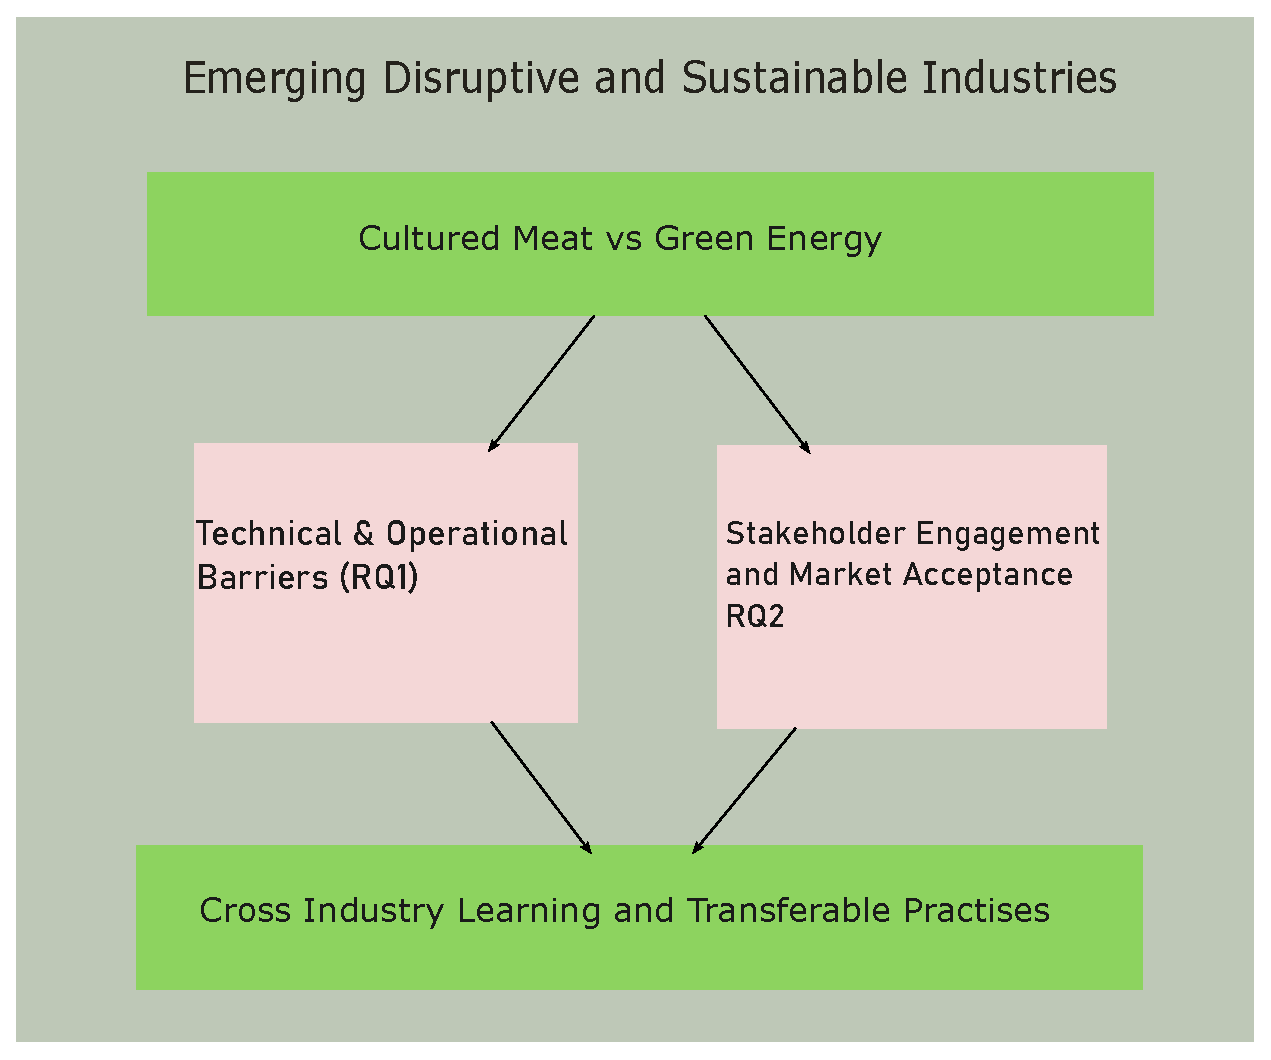
\includegraphics[width=0.9\textwidth]{images/conceptual_Model.eps}
	\caption{Conceptual Framework Guiding the Comparative Analysis.}
	\label{fig:framework}
\end{figure}

From this comparative context, the framework bifurcates into the two primary pillars of investigation, each corresponding directly to a core research question:

\begin{enumerate}
	\item \textbf{Technical \& Operational Barriers (RQ1):} This pillar guides the exploration of how management strategies differ in addressing the distinct, energy-intensive production challenges inherent to each sector. For the clean energy industry, these challenges appear as scaling existing renewable infrastructure and managing grid integration logistics. In contrast, for the nascent cultured meat industry, the barriers are more foundational, involving the optimization of novel bioreactor processes and the reduction of growth medium costs to achieve commercial viability.
	
	\item \textbf{Stakeholder Engagement and Market Acceptance (RQ2):} This pillar focuses on the role of middle management commitment in overcoming public and regulatory hurdles. In the cultured meat sector, this involves mitigating deep-seated consumer skepticism related to product novelty, naturalness, and safety. For the more established clean energy sector, the challenge shifts to securing specific regulatory buy-in for new projects and addressing community-level concerns such as NIMBYism ('Not In My Back Yard').
\end{enumerate}

The analysis of these two pillars across both industries converges towards the ultimate objective of the research: to generate \textbf{Cross-Industry Learning and Transferable Practices}. By synthesizing the findings, this study aims to develop context-specific management frameworks and provide actionable, evidence-based strategies for middle managers. This process of cross-sector learning is intended to inform both managerial practice and policy design, thereby contributing to the acceleration of sustainability transitions in these critical industries.
